\chapter{基于联邦学习的分布式缺陷检测}
\section{联邦学习框架}
\begin{figure}[htbp]
  \centering
  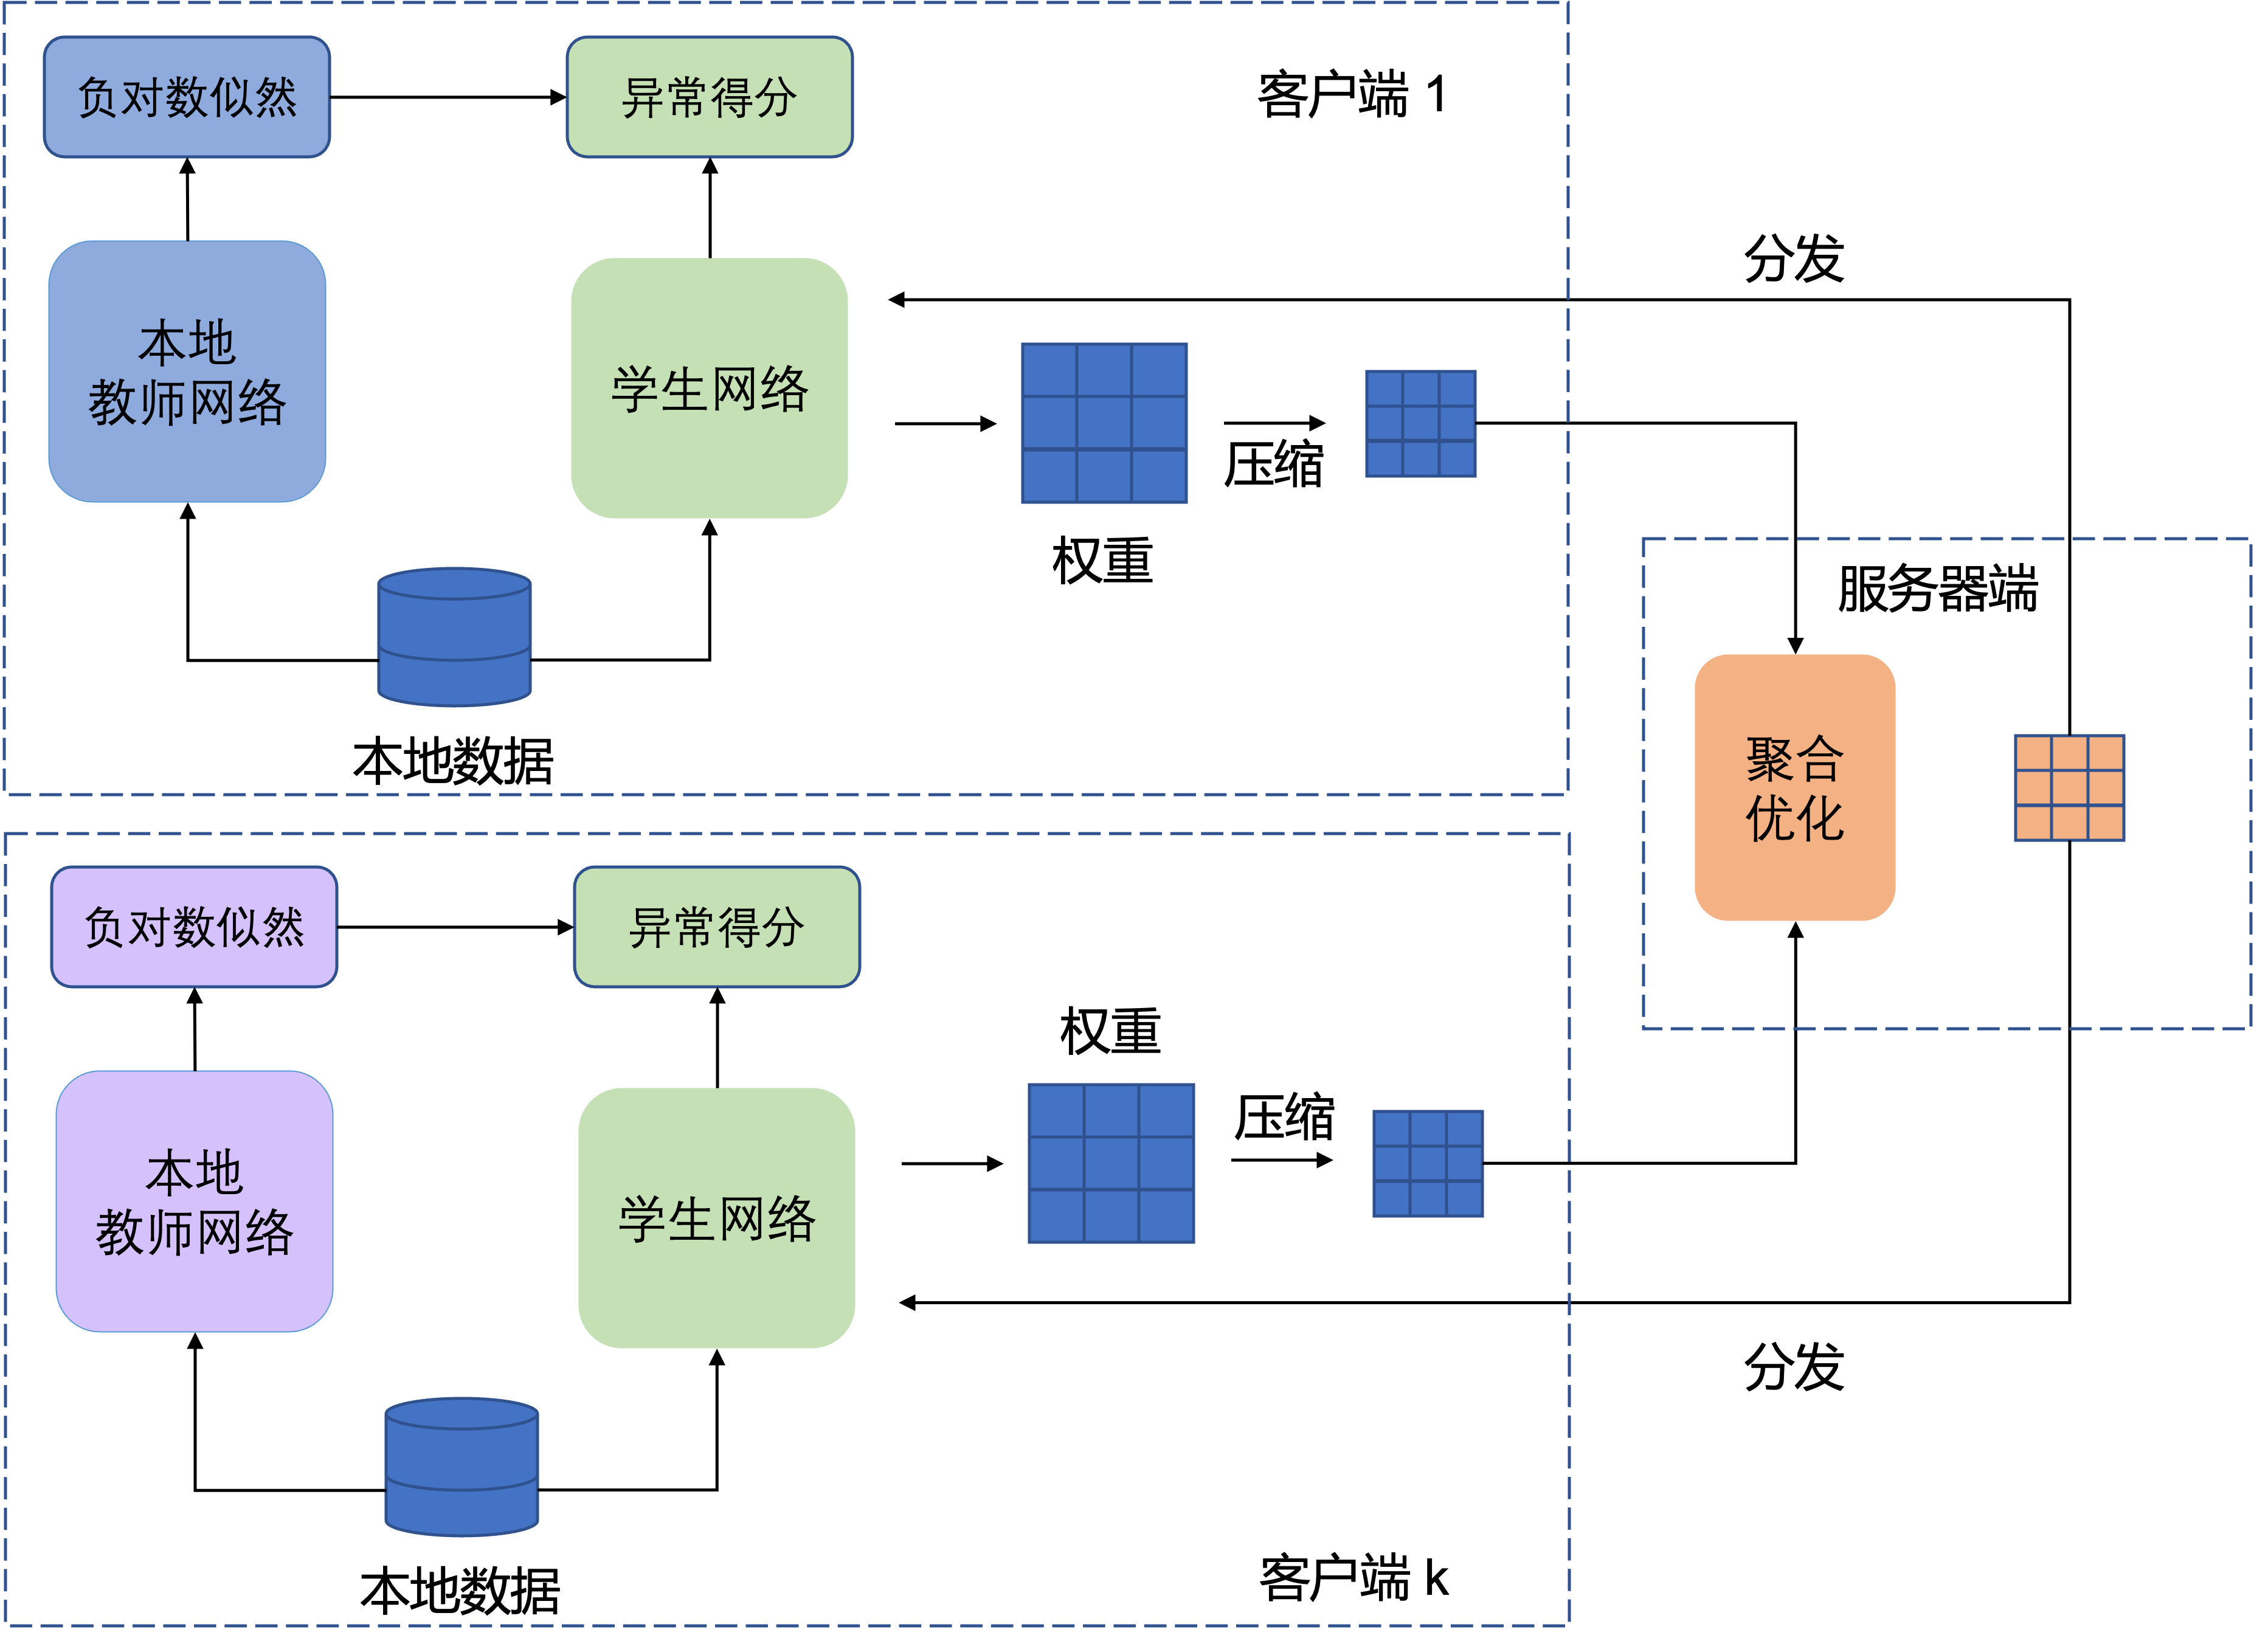
\includegraphics[width=1\textwidth]{figures/5/fed-framework.pdf}
  \caption{联邦学习框架}\label{fig:fed-framework}
\end{figure}
对于工业缺陷检测,在传统的中心化模型下,由于涉及到大量的数据收集和传输,单个中心节点往往难以满足企业对于检测实时性和私有数据隐私保护的要求。因此,近年来基于联邦学习的分布式缺陷检测逐渐受到越来越多研究者关注。

联邦学习是一种分布式学习的方法,可以在不暴露数据隐私的情况下,将各个参与者的本地数据进行训练和协同,从而达到共同提高模型性能的目的。由于参与者在本地进行训练,因此也不需要将数据传输到中心节点,系统的实时性也有所提高。此外,参与者还可以随时加入或退出,系统可以按需动态扩展。

一般来说,在联邦学习的回合中有两个参与方:客户端和服务器端。客户端持有一系列用于在每个客户端节点上训练模型并生成本地模型$\mathcal{M}=\left\{M_{1}, M_{2}, \ldots, M_{N}\right\}$ 的本地私有数据$\mathcal{D}=\left\{\mathcal{D}{1}, \mathcal{D}{2}, \ldots, \mathcal{D}_{N}\right\}$,这里N代表客户端的数量。经过本地训练过程后,本地模型M会被上传到服务器端,而不是数据D,实现聚合算法以获取全局模型$M_{global}$,其过程定义如式\ref{equ:mglobal}。

\begin{equation}\label{equ:mglobal}
  M_{\text {global }}=A G G\left(M_{1}, M_{2}, \ldots, M_{N}\right)
\end{equation}

其中AGG代表聚合算法。按上述流程即完成一轮联邦学习,然后服务器节点会将全局模型分发到每个客户端节点进行进一步的本地训练。具体的轮数通常由模型表现确定,一般当模型能够达到理想的准确性时就可以停止该过程。

在联邦学习中,m个客户端节点旨在以协作方式学习全局模型,而不彼此交换其数据点。本文目标工况为客户端节点只能通过连接到中央服务器节点交换信息而不能在客户端节点间直接交互。因此,基于联邦学习的缺陷检测算法性能很大程度上取决于服务器端的聚合算法。形式上,联邦学习的目标是优化目标函数如式\ref{equ:optimation}所示。

\begin{equation}\label{equ:optimation}
  \min _{\boldsymbol{w} \in \mathbb{R}^{d}} f(\boldsymbol{w}) \triangleq \sum_{k=1}^{m} \alpha_{k}f_{k}(\boldsymbol{w})
\end{equation}

这里w是深度神经网络的权重,$\alpha_{k}$表示第k个客户端的重要性并且$\sum_{k=1}^{m}=1$ 。在联邦学习中,聚合算法决定分配给$\alpha_{k}$的值。$f(w)$是全局损失函数。$f_{k}: \mathbb{R}^{d} \rightarrow \mathbb{R}$是客户端k对应的损失函数。这里进一步假设每个客户端节点k的本地目标函数是节点k数据点集上的期望损失,即

\begin{equation}
  f_{k}(\boldsymbol{w})=\mathbb{E}{\boldsymbol{z} \sim \mathcal{P}_{k}}\left[\ell_{k}(\boldsymbol{w}, \boldsymbol{z})\right]
\end{equation}

其中z是一个随机变量,具有概率分布$P_{k}$,损失函数$l_{k}$衡量模型的表现如何。这里将$P_{k}$视为生成数据点的客户端节点k的基础分布,而随机变量z的实现是客户端节点k的数据点。

在本文的基于异构教师学生网络的联邦学习中,每个元素样本点 $z_{j}$ 对应于一对输入(特征)向量 $x_{j}$ 和教师网络归一化的伪标签 $y_{j}$。在本例中,$\ell_{k}\left(\boldsymbol{w}, \boldsymbol{z}_{j}\right)=\ell_{k}\left(\boldsymbol{w},\left(\boldsymbol{x}_{j}, y_{j}\right)\right)$衡量模型w在预测伪标签为$y_{j}$的$x_{j}$的表现。

值得一提的是在联邦学习中客户端数据概率分布不一定相同,而根据客户端数据分布和损失函数的类别可以将联邦学习分为同构和异构。不过因为本文所有客户端节点使用的本地模型均为第四章设计的异构教师学生网络,所以客户端节点损失函数均为同构,即$\left(\ell_{1}=\ldots=\ell_{m}\right)$。因此本文联邦学习算法的同构还是异构主要取决于客户端数据分布是同构还是异构,即数据分布是$\left(\mathcal{P}_{1}=\ldots=\mathcal{P}{m}\right)$ 的IID(independently and identically distributed,独立同分布)还是不相等的non-IID。
\section{模型聚合优化}
为了防止恶意攻击者利用梯度攻击算法来窃取节点信息,客户端节点需要直接传输模型参数而不能传输梯度,联邦学习服务器节点则通过聚合所有客户端节点本地迭代更新过的网络权重到全局网络权重中来优化神经网络模型。\cite{zengFedLabFlexibleFederated2022}

在应用联邦学习进行分布式缺陷检测中,由于每个客户端节点所处的具体工况不同,客户端节点间数据分布可能是non-IID(not independently and identically distributed,非独立同分布),而未进行聚合优化的全局模型直接共享给节点会导致节点本地模型存在鲁棒性较差和收敛速度较慢的问题。因此聚合优化的目标是提高联邦学习中的全局模型的性能,从而共享给本地节点更快更鲁棒的全局模型,这同时也是联邦学习的核心输出。
\subsection{联邦平均算法}
FedAvg(Federated Averaging,联邦平均)是典型且流行的使用权重级聚合函数类型的联邦学习算法,因此本文应用FedAvg来实现基于联邦学习缺陷检测的聚合优化。在FedAvg中,客户端通过多次本地更新共享全局模型,然后将结果发送到服务器,服务器节点对本地更新的模型进行平均以计算下一个全局模型,从而实现提升通信效率,即服务器节点不对模型进行SGD,因此FedAvg也被称为本地SGD。\cite{collinsFedAvgFineTuning2022,mcmahanCommunicationEfficientLearningDeep2023}

SGD(Stochastic Gradient Descent,随机梯度下降)是一类常见的优化算法,通常用于神经网络模型训练中。它是梯度下降算法的一类变体,每次更新网络权重时,只使用数据集中采样的部分样本而不是整个数据集,这样可以减少计算量并加速模型训练。根据采样数量SGD可以分为批量采样的Batch-SGD、小批量采样的Mini-Batch SGD以及单个样本的SGD,本文不特别说明采样类别时提到的SGD是对随机梯度下降方法的统称。

在FedAvg的每一轮客户端节点与服务器节点通讯t中,服务器会随机地从m个客户端中采样一个客户端子集$\mathcal{S}_{t}$。每个被选中的客户端节点都会收到当前的全局模型参数$w_{t}$,客户端节点将$w_{t}$载入本地模型并开始在其本地数据上执行多个SGD优化的本地模型训练更新,然后将结果发送回服务器节点,服务器计算$w_{t+1}$作为更新的全局模型参数。其算法流程详见算法\ref{alg:FedAvg}。

\begin{algorithm}[H]
  \SetAlgoLined
  \KwIn{通过k索引K个客户端;小批尺寸 B;本地迭代更新总轮数 $\tau$;学习率 $\eta$ }
 
  \KwOut{ 全局模型参数 $w$ }
  
  \SetKwFunction{FMain}{in parallel}
  \SetKwFunction{Fupdate}{ClientUpdate}
  \SetKwProg{Fn}{服务器执行}{:}{客户端本地微调}
  \Fn{}{初始化 $w_{0}$\\
        \ForEach{通讯轮$t = 1,2,...$}{
          $m \longleftarrow max(C·K,1)$\\
          $S_{t} \longleftarrow (m \text{个客户端随机采样的子集})$\\
          \ForEach{$k \in S_{t}$ \FMain}{
            $w^{k}_{t+1} \longleftarrow $ \Fupdate{$k,w_{t}$}
          }
          $m_{t} \longleftarrow \sum_{k \in \mathcal{S}_{t}} n_{k}$\\
          $w_{t+1} \longleftarrow  \frac{1}{m_{t}} \sum_{k \in \mathcal{S}_{t}} n_{k}\boldsymbol{w}^{k}_{t+1,\tau}$
        }
  }
  \SetKwProg{Fc}{Function}{:}{Return{ $w$}}
  \Fc{\Fupdate{$k,w$}}{
    $\mathcal{B} \longleftarrow (\text{将本地数据集划分为批集合,批大小为} B) $\\
    \ForEach{$i$ in $range(0,\tau-1)$}{
      \ForEach{$b\in\mathcal{B}$}{
        $w \longleftarrow w - \eta \bigtriangledown \ell(w;b)$
      }
    }
  }
  \caption{联邦平均算法}\label{alg:FedAvg}
 \end{algorithm}

具体而言,在接收全局模型参数$w_{t}$后,客户端节点k第i+1轮本地模型迭代更新的网络权重$\boldsymbol{w}^{k}_{t, i+1}$的计算公式如式\ref{equ:wcal}所示

\begin{equation}\label{equ:wcal}
  \boldsymbol{w}^{k}_{t, i+1}=\boldsymbol{w}^{k}_{t,i}-\eta \bigtriangledown^{(k)} \ell\left(\boldsymbol{w}^{k}_{t,i}\right)
\end{equation}


其中i = 0, . . . , τ − 1,  τ是本地迭代更新轮数,当i = 0时,$\boldsymbol{w}^{k}_{t, 0}=\boldsymbol{w}_{t}$。$\eta$ 是学习率,$\bigtriangledown^{(k)} \ell\left(\boldsymbol{w}^{k}_{t, i}\right)$是客户端节点k从本地数据集中按B的批尺寸划分的批集合中元素b在网络权重为$w^{k}_{t,i}$的模型上评估损失函数$\ell(·)$的随机梯度。

当$\boldsymbol{w}^{k}_{t, i+1} = \boldsymbol{w}^{k}_{t, \tau}$时  ,即客户端节点k本地更新完成,节点随即上传本地模型参数$\boldsymbol{w}^{k}_{t,\tau}$至服务器节点。待所有客户端节点均上传本地模型参数至服务器节点后,由服务器节点计算全局聚合优化模型参数并分发给客户端节点,用于下一轮客户端进行本地模型参数初始化。全局聚合优化公式如式\ref{equ:globalopti}所示。

\begin{equation}\label{equ:globalopti}
  \boldsymbol{w}_{t+1}=\frac{1}{m_{t}} \sum_{k \in \mathcal{S}_{t}} n_{k}\boldsymbol{w}^{k}_{t,\tau}
\end{equation}

其中$n_{k}$是客户端节点k所对应的本地数据集样本个数,$m_{t}:=\sum_{k \in \mathcal{S}_{t}} n_{k}$。当本地迭代更新轮数$\tau=1$时,FedAvg就等价为D-SGD(Distributed-SGD,分布式随机梯度下降),也被称为mini-batch SGD(小批量随机梯度下降),其收敛性质已经在多个研究中的被验证。FedAvg则是通过在服务器与客户端节点相邻通信轮之间进行τ≥2次的客户端本地更新来提高D-SGD的通信效率。

\subsection{模型微调}
当客户端节点的数据相似时,每个节点采用多轮本地更新的方法可以改善所有其他客户端数据上的模型性能,因此在具有同构数据的客户端节点中,FedAvg表现良好。不过,在更现实的异构数据设置中,需要在经过FedAvg多轮本地训练更新共享的全局模型后,再对单个客户端节点进行微调,来使其在异构联邦学习设定下也表现良好。

经过T轮服务器和客户端节点通讯后,并将FedAvg方法聚合优化的全局模型参数 $w_{T}$ 应用于客户端节点本地任务前,通常会在每个客户端节点上再对模型进行微调。具体来说,将服务器上的全局模型参数 $w_{T}$ 下载到所有客户端节点,客户端节点k 按式\ref{equ:sgdw}对其本地数据执行 $\tau^{\prime}$步 SGD:

\begin{equation}\label{equ:sgdw}
  \boldsymbol{w}^{k}_{T, i+1}=\boldsymbol{w}^{k}_{T,i}-\eta \bigtriangledown^{(k)} \ell\left(\boldsymbol{w}^{k}_{T,i}\right),i \in\left[\tau^{\prime}-1\right]
\end{equation}

微调后的模型参数$\boldsymbol{w}_{T, i, \tau^{\prime}}$将最终用于本地客户端节点对应的任务。如果有新客户端节点在FedAvg整个训练完成后进入系统,其索引为K + 1,也可以使用相同的过程微调$w_{T}$ ,以获得个性化的本地模型参数 ${w}^{K+1}_{T,\tau^{\prime}}$。

  

\section{联邦通信压缩}
在应用联邦学习于工业缺陷检测时,跨空间进行协同的设备通讯条件不一,这可能导致通信成本非常高,成为制约扩展分布式优化算法的瓶颈之一。因此在对通讯成本敏感的工况下,降低联邦学习通讯的负载必不可少。

本文利用知识蒸馏的方式,在本地训练模型参数相对较大的教师模型,通过教师模型训练模型相对简单的学生模型,将较小的学生模型参数作为本地客户端节点与服务器节点间通讯的负载,从而有效降低通讯所需带宽。

虽然通过本地训练教师学生网络输出的模型参数已经较小,但是为了进一步降低联邦学习中的总体通讯开销,本文在联邦平均算法的基础上引入了模型量化的方法,在传输消息时采用量化算子,根据量化器的精度,通过交换量化的更新来减少模型参数上行通信的开销。本文研究的对象是客户端节点的网络模型同构,数据分布为non-IID的情况,因此各客户端节点模型量化方法一致。

具体来说,在客户端节点和服务器通讯的第t轮,客户端节点k的τ本地迭代更新的输出为$\boldsymbol{w}_{t,\tau}^{k}$,不同与直接上传到服务器节点,模型量化的方法对每个客户端节点进行量化压缩处理$Q(\cdot)$,然后客户端节点再上传压缩信号到服务器节点。

压缩的信号$\boldsymbol{\Delta}_{t}^{k} \triangleq Q\left(\left(\boldsymbol{w}_{t,\tau}^{k}-\boldsymbol{w}_{t}^{k}\right) / \eta
\right)$表示在节点k处第t轮本地SGD过程的输入和输出之间差异的标准化版本,它等于客户端节点所有本地SGD方向的聚合,即$\left(\boldsymbol{w}_{t,\tau}^{k}-\boldsymbol{w}_{t}^{k}\right) / \eta =\sum_{i=0}^{\tau} \mathbf{g}_{t,i}^{k}$。

当服务器节点收到所有客户端节点的压缩信号,$\left\{\boldsymbol{\Delta}_{t }^{k}\right\}_{k=1}^{j=m}$,服务器节点按式\ref{equ:wglobal}x计算全局聚合优化的模型。

\begin{equation}\label{equ:wglobal}
  \boldsymbol{w}_{t+1}=\boldsymbol{w}_{t}-\frac{\eta \gamma}{m} \sum_{k=1}^{m} \boldsymbol{\Delta}_{t}^{k}
\end{equation}

其中 $\gamma$是全局学习率,将新的全局模型变为前一个全局模型和更新的本地模型平均值的线性组合,合理的$\gamma$可以提高凸和非凸设定的复杂度界限。上式也可以解释为通过以步长$\eta\gamma$朝向聚合本地梯度方向的平均值来运行主模型的全局SGD更新。\cite{haddadpourFederatedLearningCompression2021}

本文使用的量化压缩处理$Q(\cdot)$方法为广泛使用的随机量化。\cite{reisizadehFedPAQCommunicationEfficientFederated2020}对于任意变量$\mathbf{x} \in \mathbb{R}^{p}$ ,低精度量化器$Q^{L P}: \mathbb{R}^{p} \rightarrow \mathbb{R}^{p}$的定义如式\ref{equ:qlp}所示。 

\begin{equation}\label{equ:qlp}
  Q_{i}^{L P}(\mathbf{x})=\|\mathbf{x}\| \cdot \operatorname{sign}\left(x_{i}\right) \cdot \xi_{i}(\mathbf{x}, s), \quad i \in[p]
\end{equation}


其中$\xi_{i}(\mathbf{x}, s)$是一个随机变量,以$\frac{\left|x_{i}\right|}{\|\mathbf{x}\|} s-l$的概率取值为$\frac{l+1}{s}$,否则取值为$\frac{l}{s}$。这里,调整参数s对应于量化级别的数量,$l \in[0, s)$是一个整数,使得$\frac{\left|x_{i}\right| }{ \|\mathbf{x}\|} \in[ \frac{l}{s} , \frac{ l+1 }{s})$。


\section{联邦学习仿真}
联邦学习的最终应用场景是分布式多节点,为了在前期快速验证算法可行性,本文利用联邦学习框架FedLab开展本章的分布式多节点仿真。FedLab基于Pytorch的分布式API开发,标准化了联邦学习模拟的过程,包括同步算法、异步算法和通信压缩等。\cite{zengFedLabFlexibleFederated2022}此外该框架还提供了模块化工具以及联邦学习的标准化实现来提升联邦学习实验开发效率,框架原理如图\ref{fig:fedlab-overview}所示
\begin{figure}[htbp]
  \centering
  \includegraphics[width=0.75\textwidth]{figures/5/fedlab.pdf}
  \caption{FedLab框架原理}\label{fig:fedlab-overview}
\end{figure}

其中Server为服务器节点,通常仅一个;Client为客户端节点,数量由用户决定。每个节点均包含一个网络管理器(NetworkManager)和网络权重处理器,网络管理器模块管理消息处理任务,提供了定制通信协议和压缩的接口,网络权重处理器即后端计算,分为服务器的PSHandler和客户端的Trainer,其对象是模型参数。

本文的本地训练模型是第四章提到的面向多模态缺陷检测的异构教师学生(AST)网络,因此本文继承FedLab的客户端训练器类(Trainer)开发了AST的训练器类,其中基于归一化网络的教师网络仅在本地训练更新,不与服务器节点和其它客户端节点直接产生交互;每轮通信过程,学生网络将模型参数上传至服务器用于聚合并且接收服务器的全局更新后的模型。在服务器端,本文继承服务器类(PSHandler)开发了适配缺陷检测网络的评估函数,服务器节点的聚合函数本文使用FevAvg的模型聚合方法。

\begin{figure}[htbp]
  \centering
  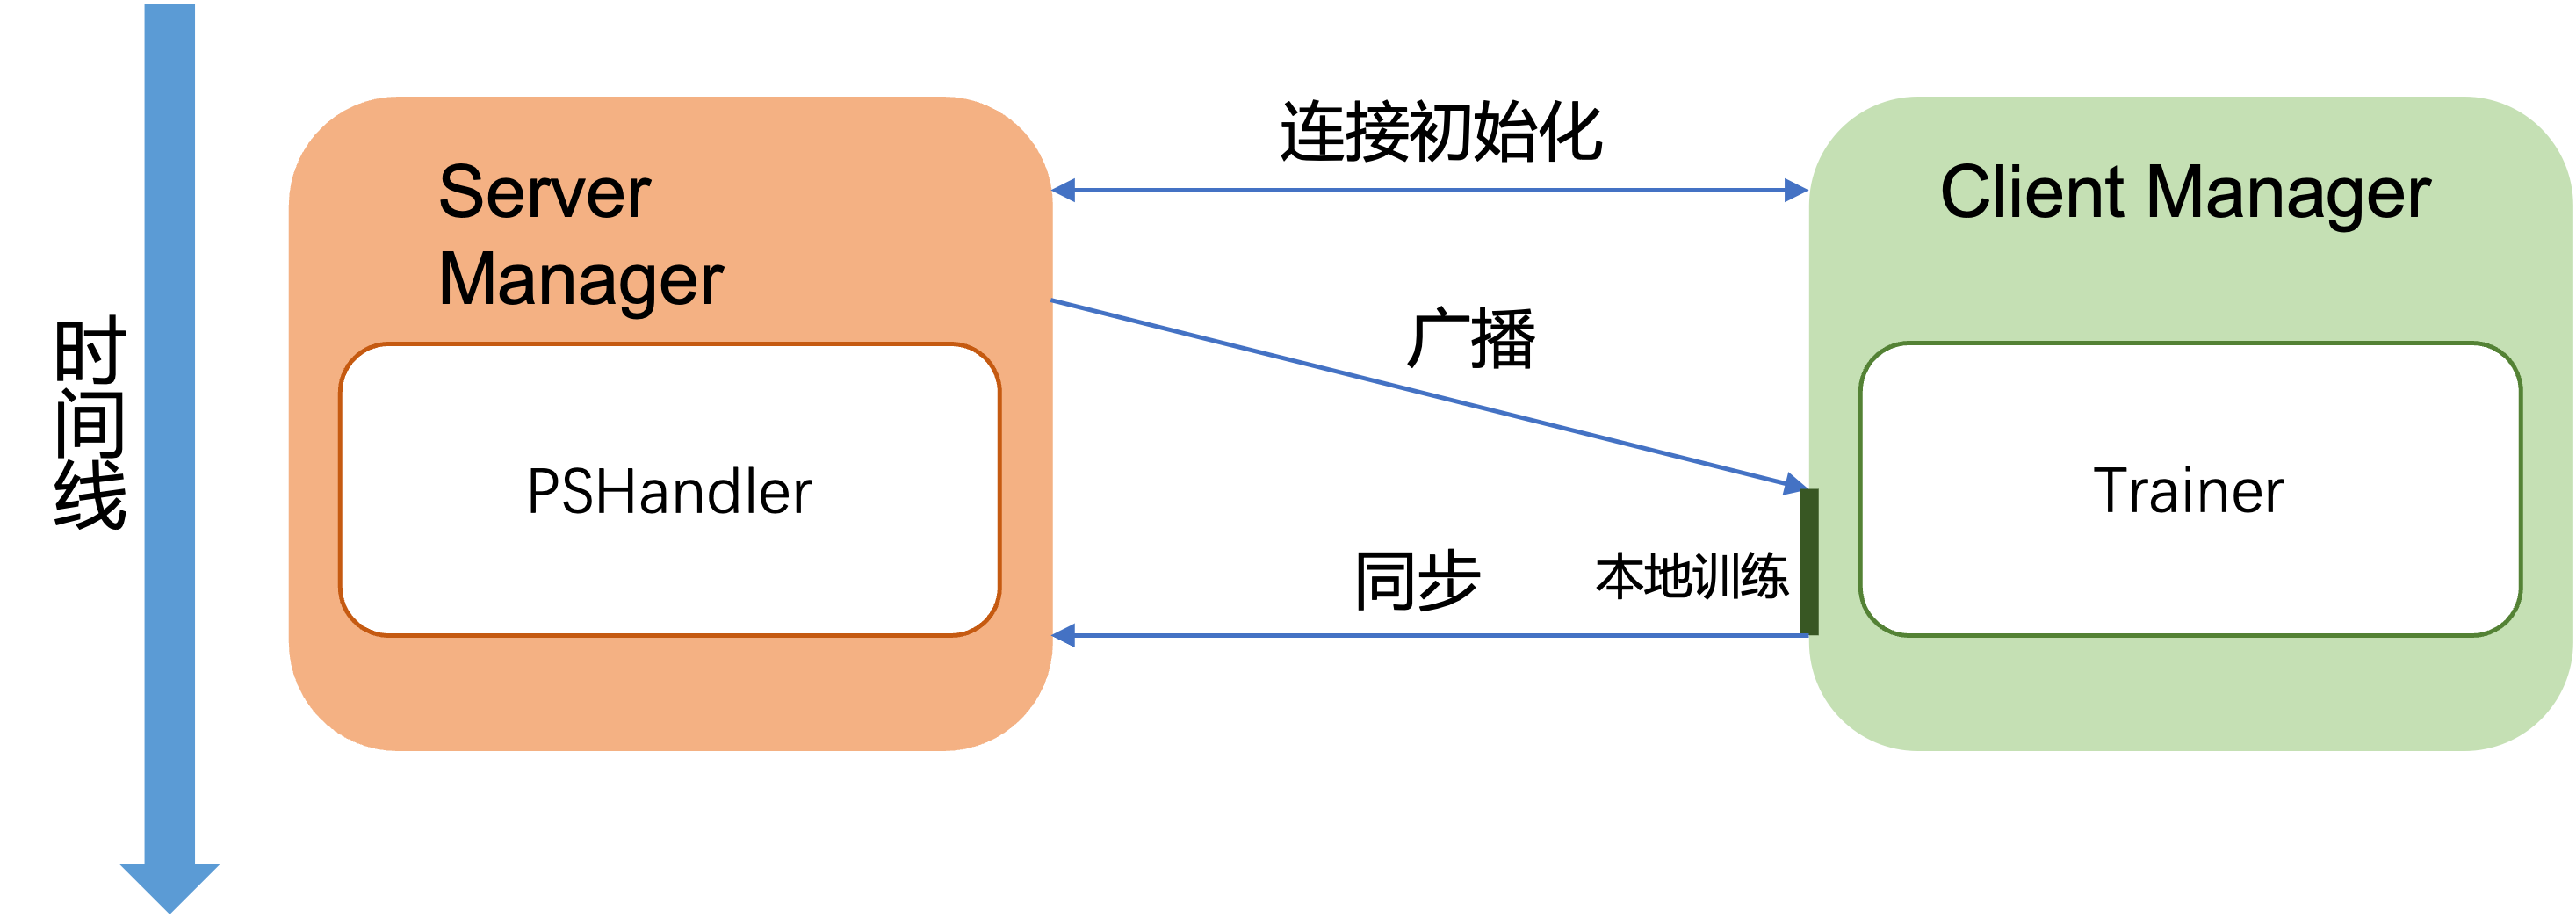
\includegraphics[width=0.8\textwidth]{figures/5/synchronous.pdf}
  \caption{FedLab框架原理}\label{fig:fedlab-synchronous}
\end{figure}
本文客户端和服务器的通信方式采用同步联邦的方式,每一轮训练由服务端开启,即服务端先随机采样客户端,并将全局模型广播给被选中的客户端;客户端收到后,执行本地训练,结束后向服务端同步本地信息,其原理如图\ref{fig:fedlab-synchronous}所示

\begin{figure}[htbp]
  \centering
  \includegraphics[width=0.75\textwidth]{figures/5/SerialTrainer.pdf}
  \caption{FedLab框架原理}\label{fig:fedlab-SerialTrainer}
\end{figure}
本文在单机单进程下使用串行训练器对联邦学习的分布式状态进行模拟仿真,其原理如图\ref{fig:fedlab-SerialTrainer}所示。对应服务器选中的虚拟客户端节点的数据集依次输入串行训练器开展本地训练,每个数据集训练结束后向服务器侧上传模型参数,然后串行训练器将模型参数重置为本轮初始网络权重再进行下一个数据集的本地训练,从而模拟多个客户端节点。


服务器节点收到模型参数后暂存,待所有选中的虚拟客户端节点对应的数据集均通过串行训练器上传完模型参数后再执行模型聚合,全局模型更新完成后再传回串行训练器用于下一轮本地训练。

\section{实验设计及结果分析}
在本节中将使用MVTec发布的3D-AD数据集进行实验分析。该数据集包含10种物体的高精度深度图和RGB图像组合,共计4147组数据。同时,数据集包含用于训练的正常样本和用于评估算法的标注缺陷。因此这个数据集适合用于模拟联邦学习缺陷检测不同产线的数据采样。本文利用该数据集开展实验,来验证基于联邦学习的AST算法在不同的产线上分布式进行缺陷检测的效果。
%TODO MVTec-3d的样本图片

本节首先设计基于联邦学习的分布式缺陷检测实验,记为实验甲,实验甲的训练参数设置如表\ref{tab:ast-fed-category}所示,
%TODO 实验甲网络权重表格
\begin{table}[htbp]
  \centering
  \caption{联邦学习缺陷检测部分超参数} \label{tab:ast-fed-category}
  \begin{tabular*}{0.75\textwidth}{@{\extracolsep{\fill}}cccc}
  \toprule
    超参数			&数值		 \\
  \midrule
    客户端节点数(client num) &  $4$    \\
    随机采样率(sample ratio)			&$1$		 \\
    通讯轮数(round)	&$9$	 \\
    本地训练轮数(epoch)	& $24$\\
    学习率(learning rate)	& $0.1$\\
    批大小(batch size)&  $8$    \\
  \bottomrule
  \end{tabular*}
\end{table}

实验甲设置4个客户端,数据分布设定为一类non-IID,即每个客户端只接受单个类别的正常样本集。\cite{zhaoFederatedLearningNonIID2022}服务器随机采样率设置为1(所有客户端都参与),通讯轮数设置为9,每个客户端节点的训练轮次为24,学习率为 ,批大小为。4个客户端节点随着轮次迭代的损失如图\ref{fig:4-client}所示
\begin{figure}[htbp]
    \centering
    \begin{subfigure}
        \centering
        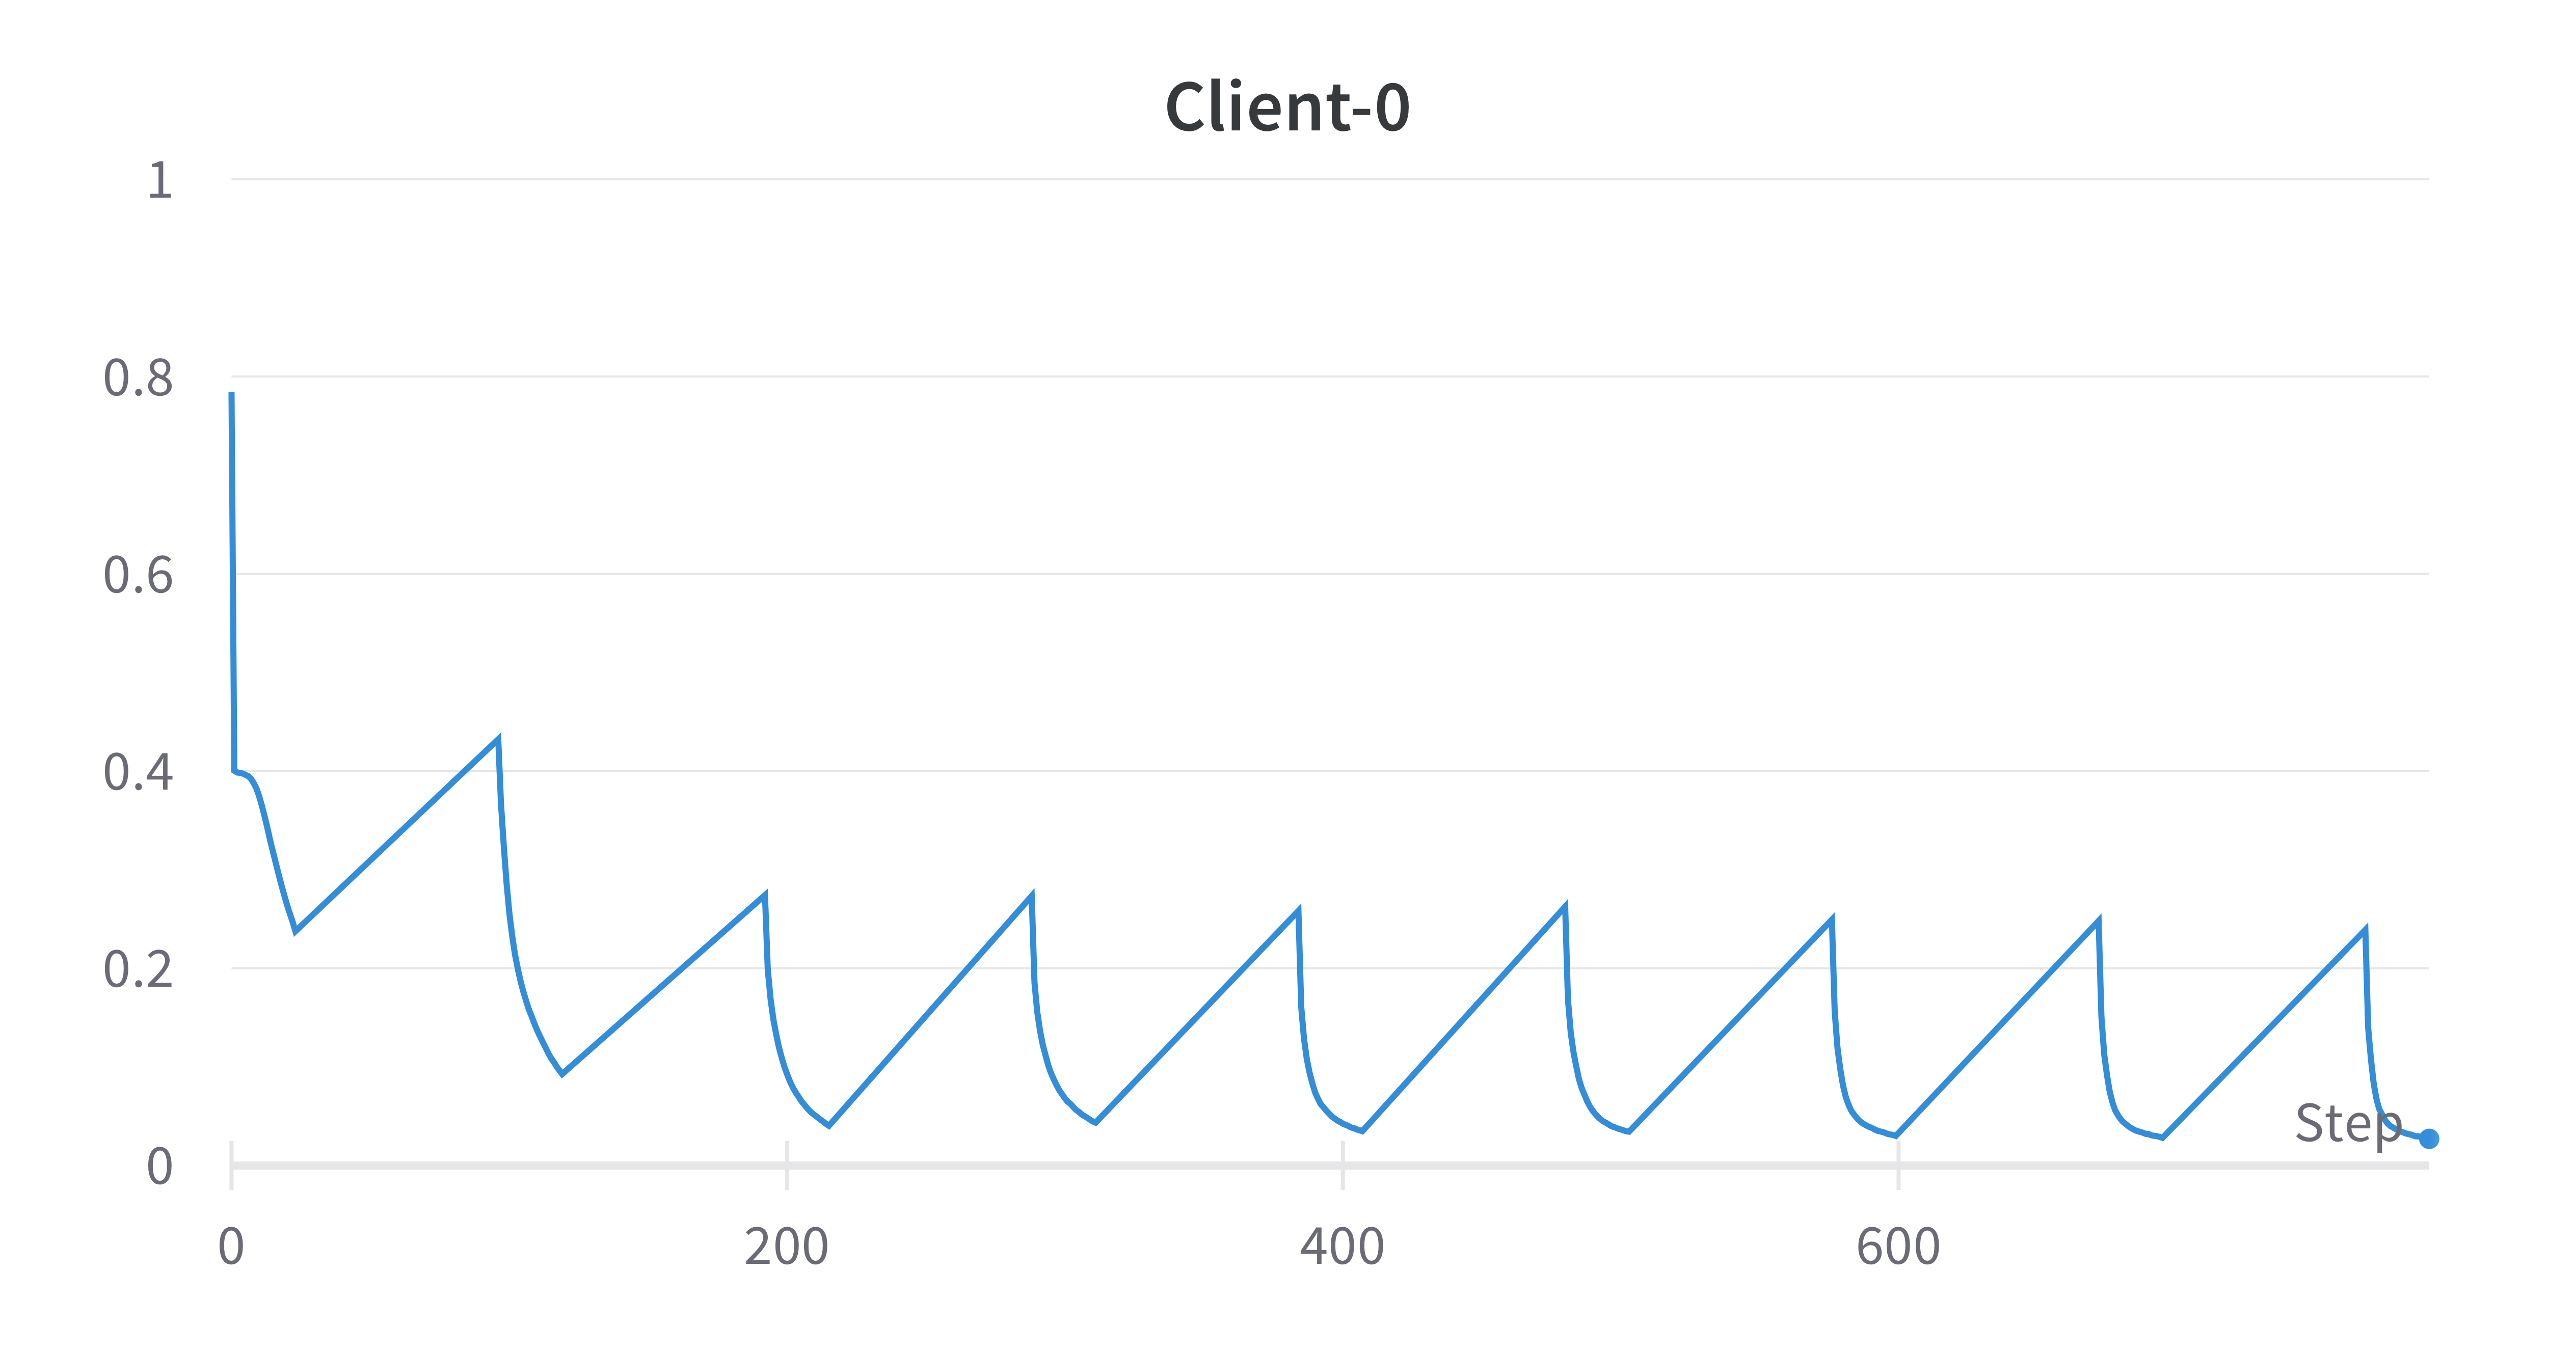
\includegraphics[width=.4\linewidth]{figures/4-client/Client-0.png}  
      \end{subfigure}
      \begin{subfigure}
        \centering
        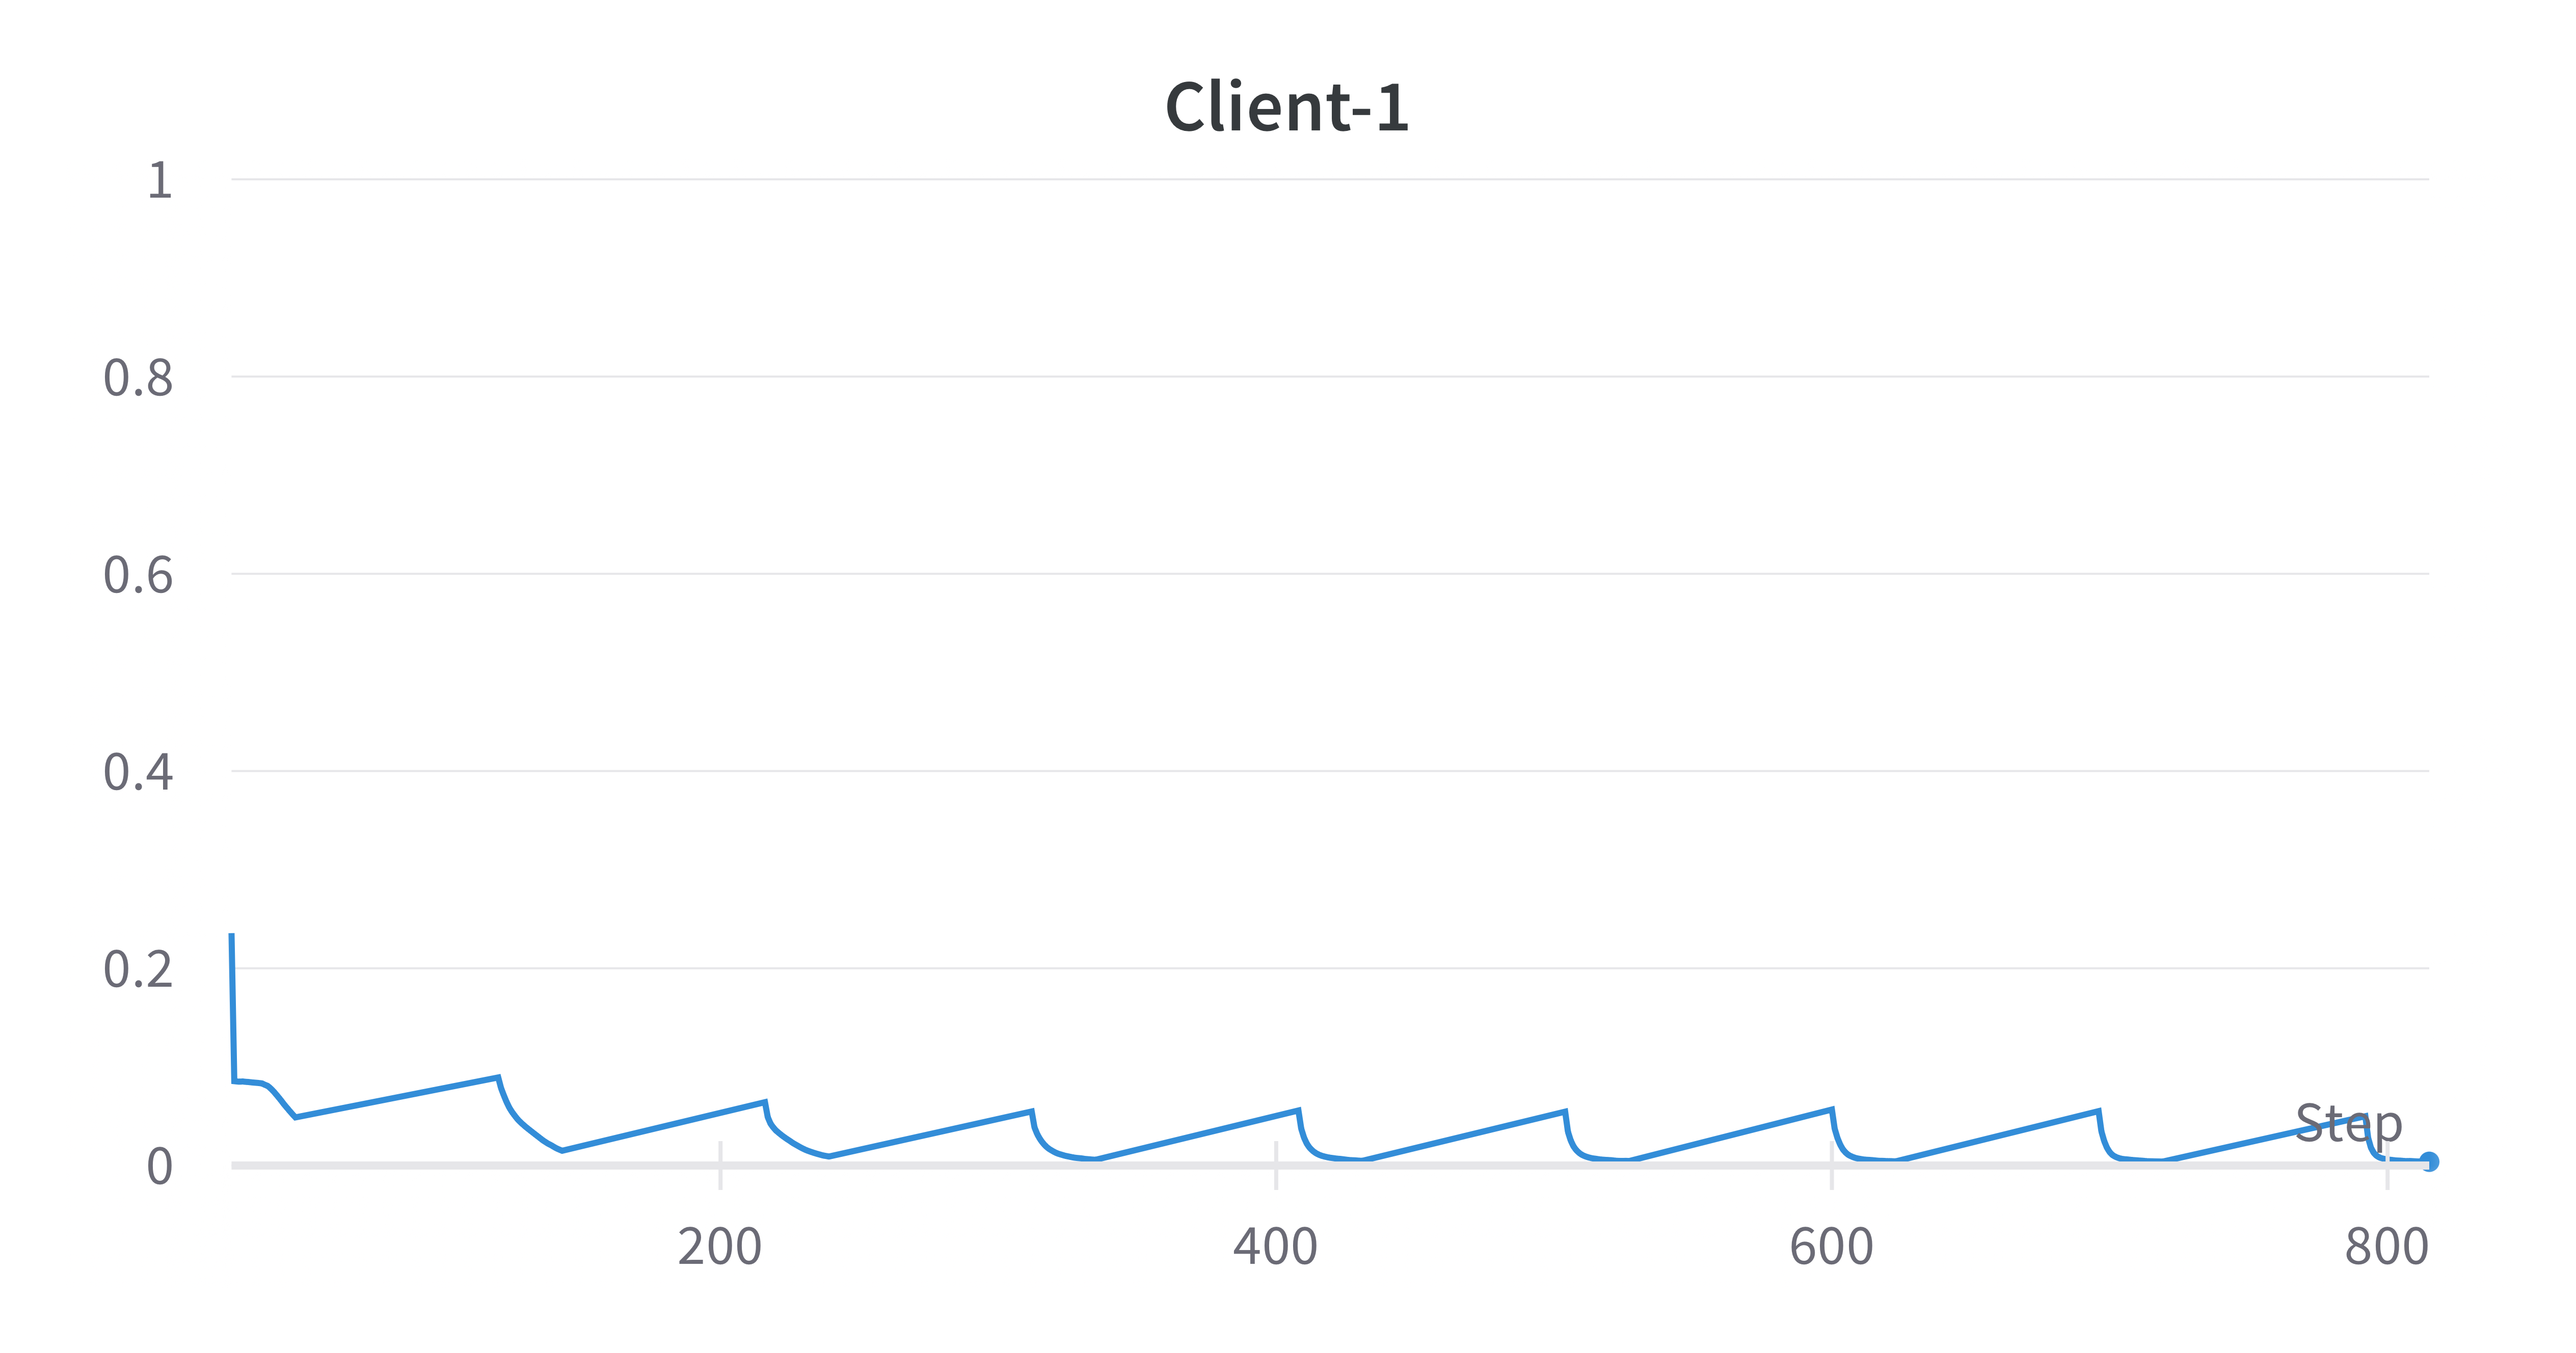
\includegraphics[width=.4\linewidth]{figures/4-client/Client-1.png} 
      \end{subfigure}
      \begin{subfigure}
        \centering
        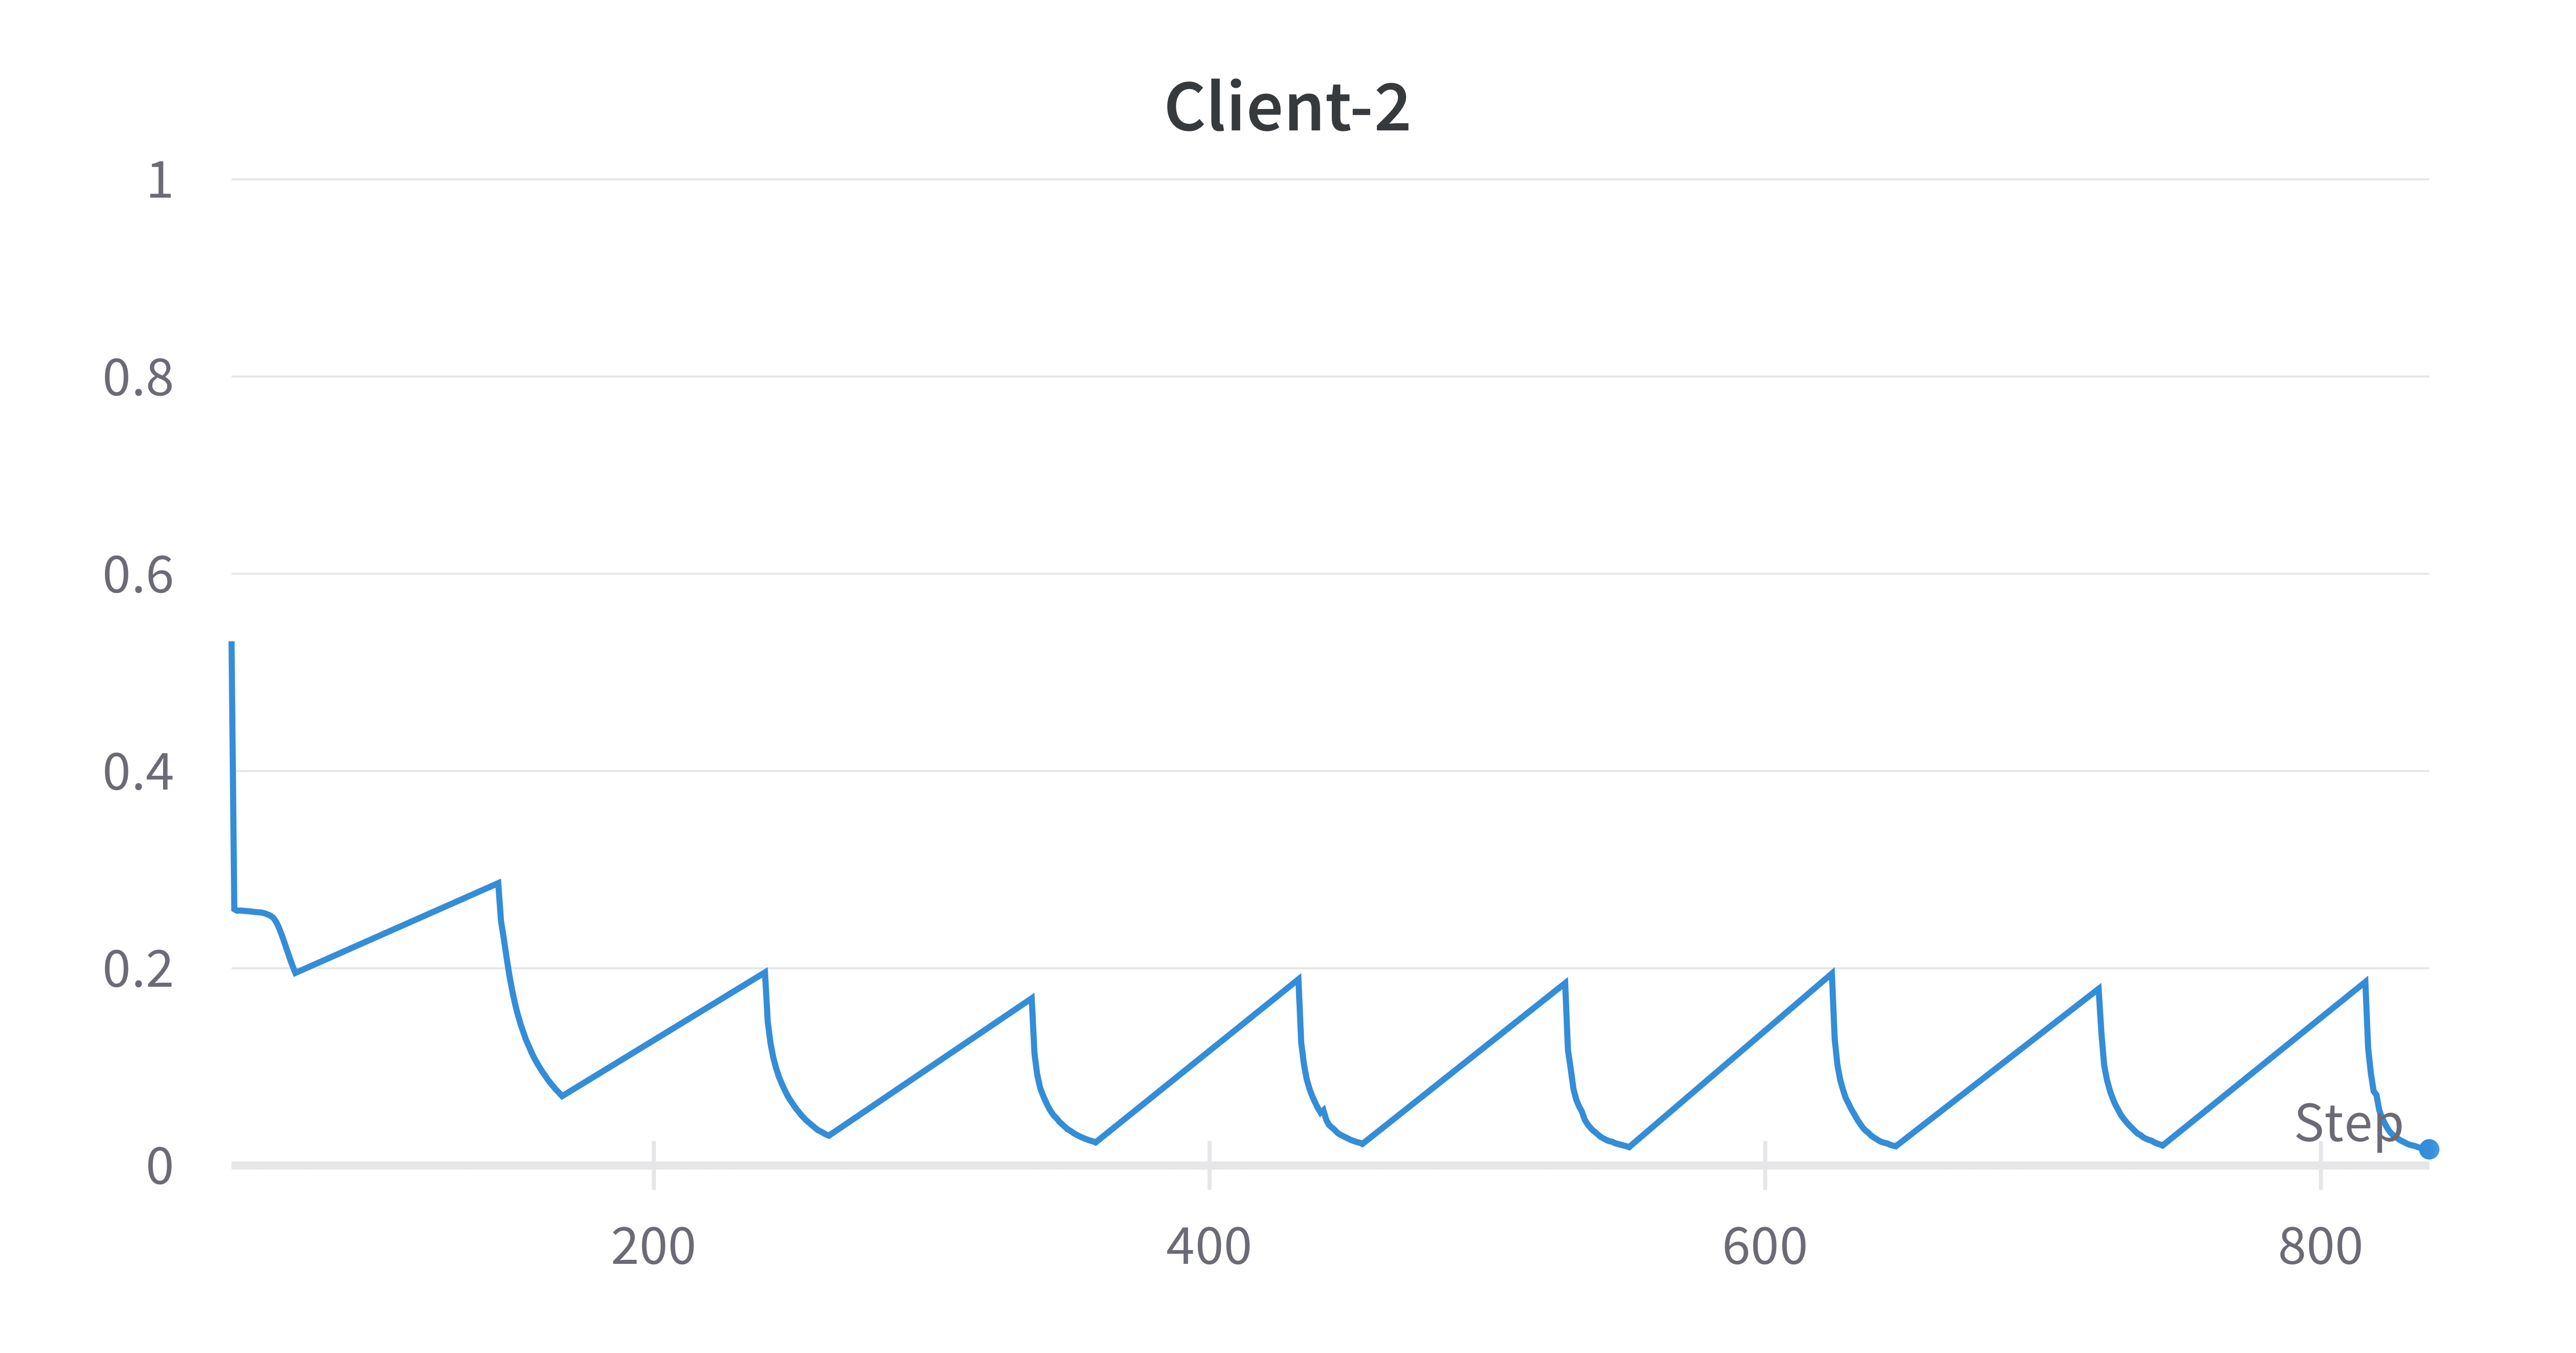
\includegraphics[width=.4\linewidth]{figures/4-client/Client-2.png}  
      \end{subfigure}
      \begin{subfigure}
        \centering
        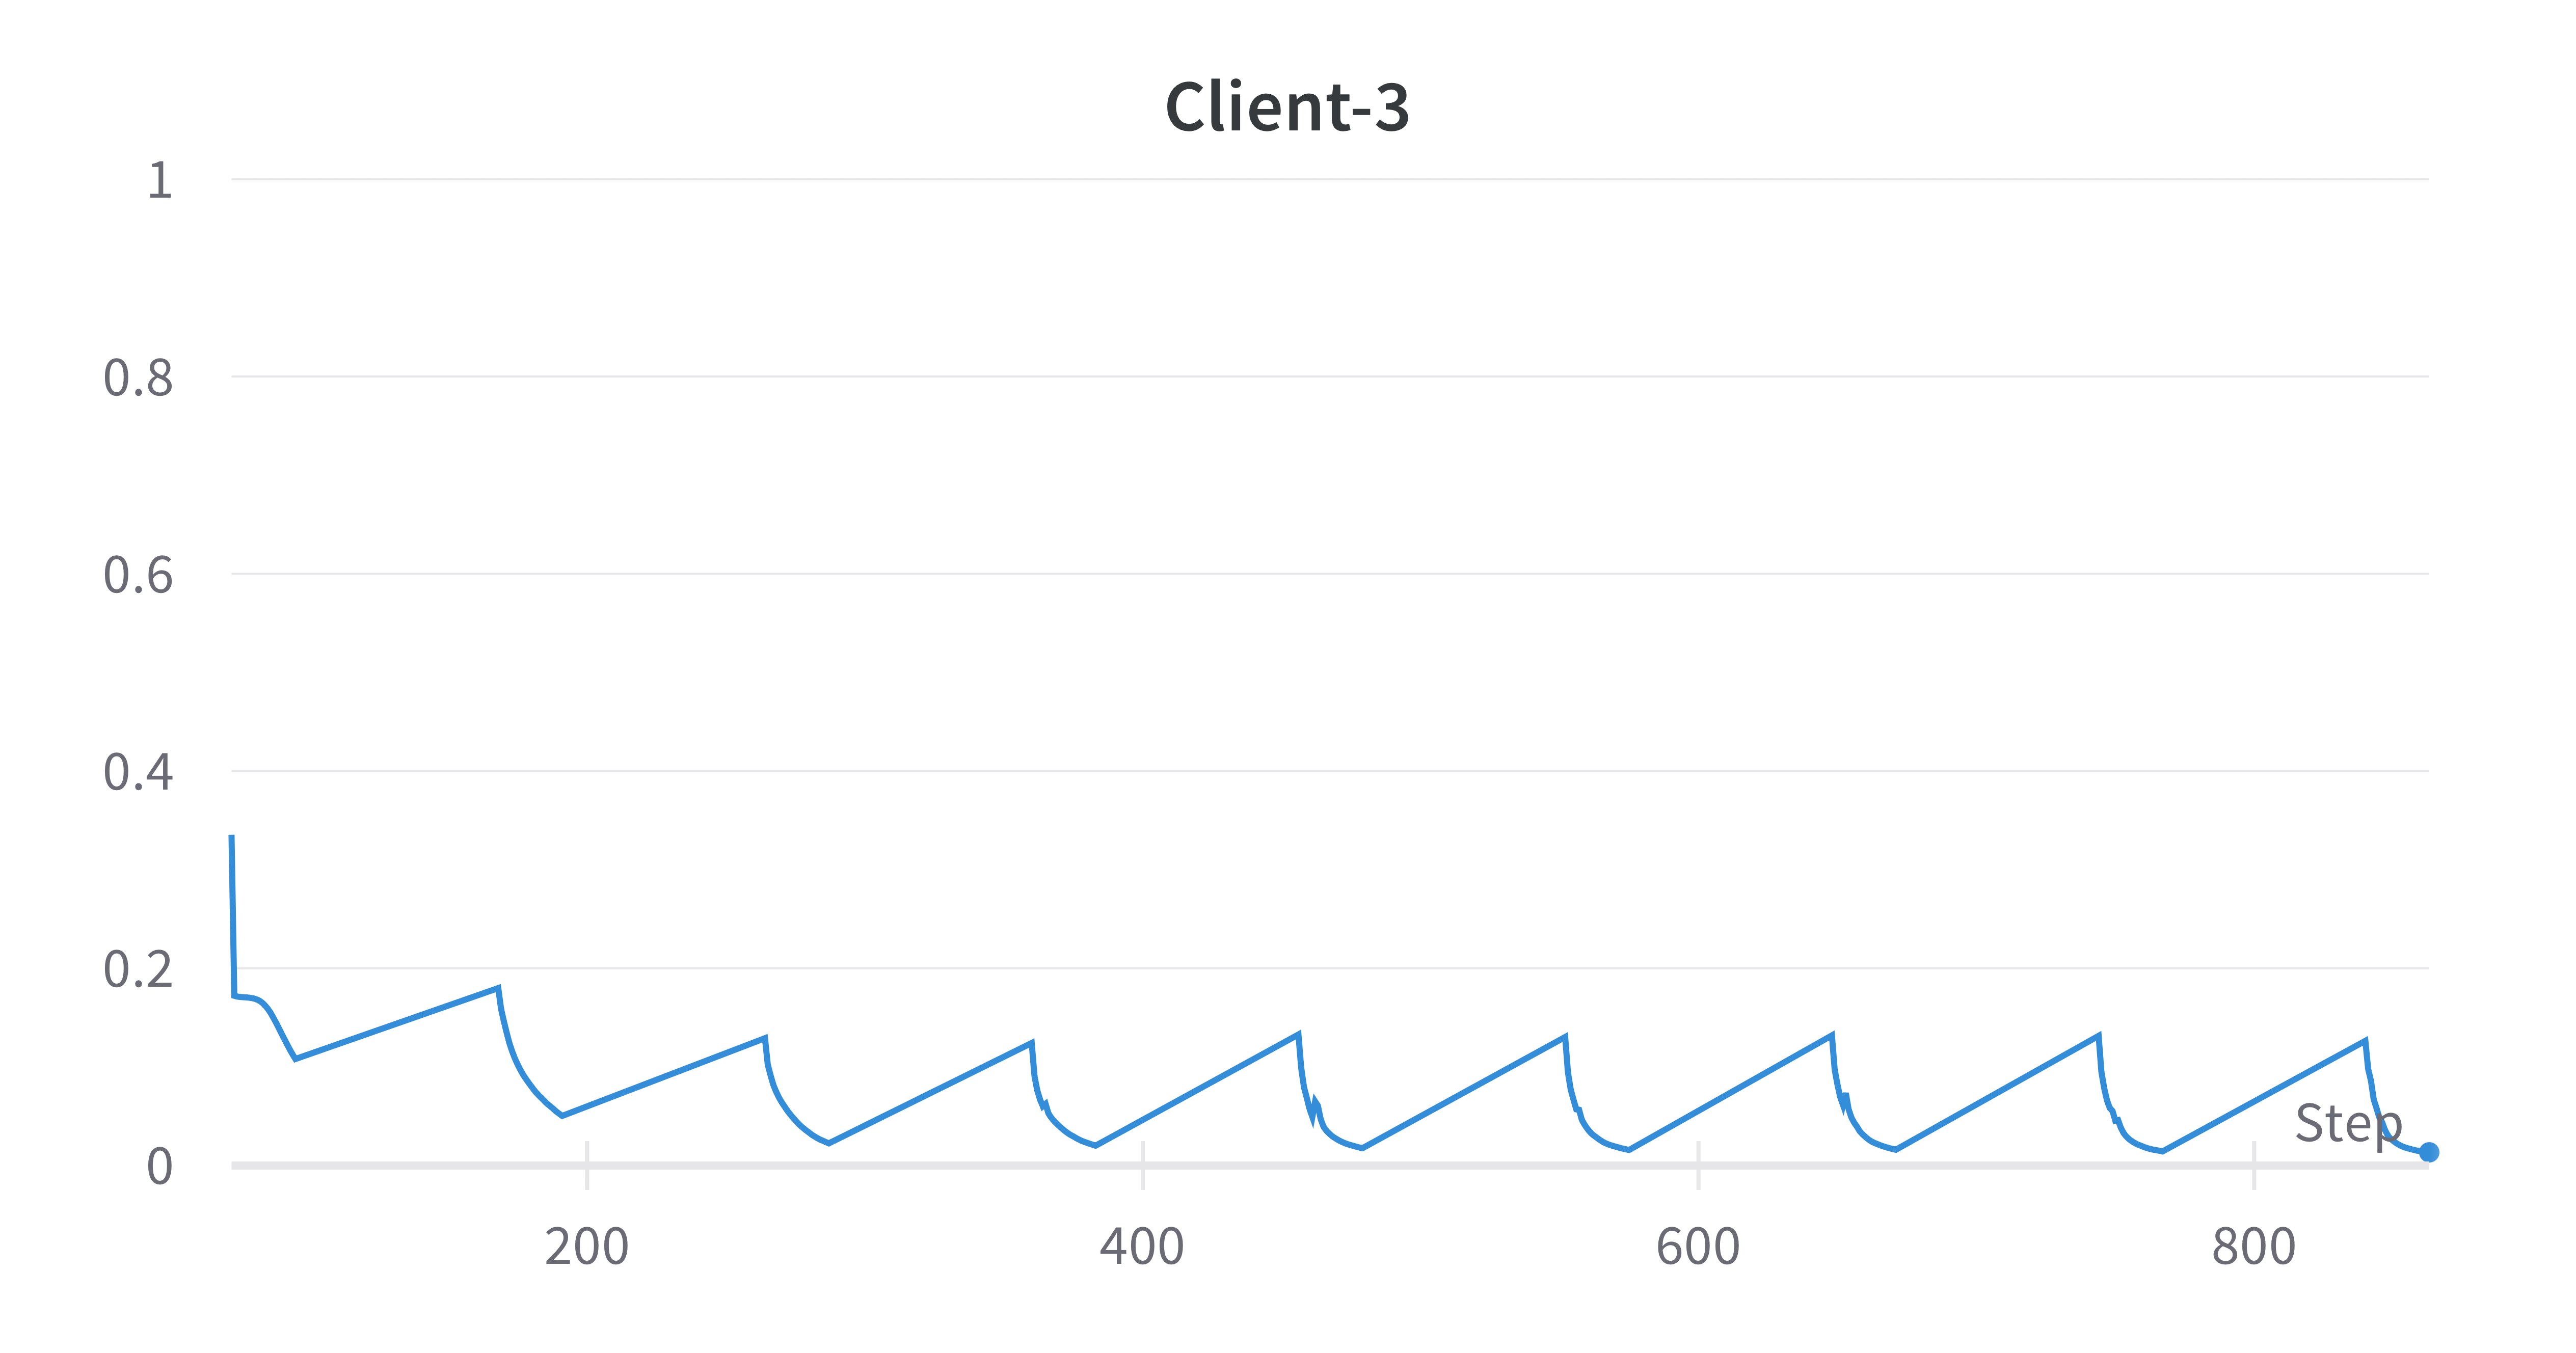
\includegraphics[width=.4\linewidth]{figures/4-client/Client-3.png} 
      \end{subfigure}
    \caption{客户端损失}
    \label{fig:4-client}
\end{figure}

图中横轴为训练的轮次,纵轴为损失值,每个折线的凸点表示对应客户端节点接收到服务端全局聚合更新模型后开始本地训练时的损失。不难看出,基本在经过3次全局聚合更新后,所有本地客户端节点收到更新模型后的损失波动很小,基本趋于收敛。该组图像也表明本文提出的异构教师学生网络联邦学习算法是可行的。

为了验证联邦学习全局模型的泛化能力,本节在联邦学习仿真实验的基础上设计了验证实验,记为实验乙。当实验甲进行到第四轮通讯时,损失已经收敛,因此实验乙与实验甲不同之处就在于此时实验乙引入一个新的客户端节点和对应新的类别数据集,用于模拟新缺陷检测产线加入,该节点的模型初始化为本轮通信中服务器节点向各客户端节点下发的已经收敛的全局聚合更新模型。实验乙效果如图\ref{fig:add-5-client}所示。
\begin{figure}[htbp]
  \centering
  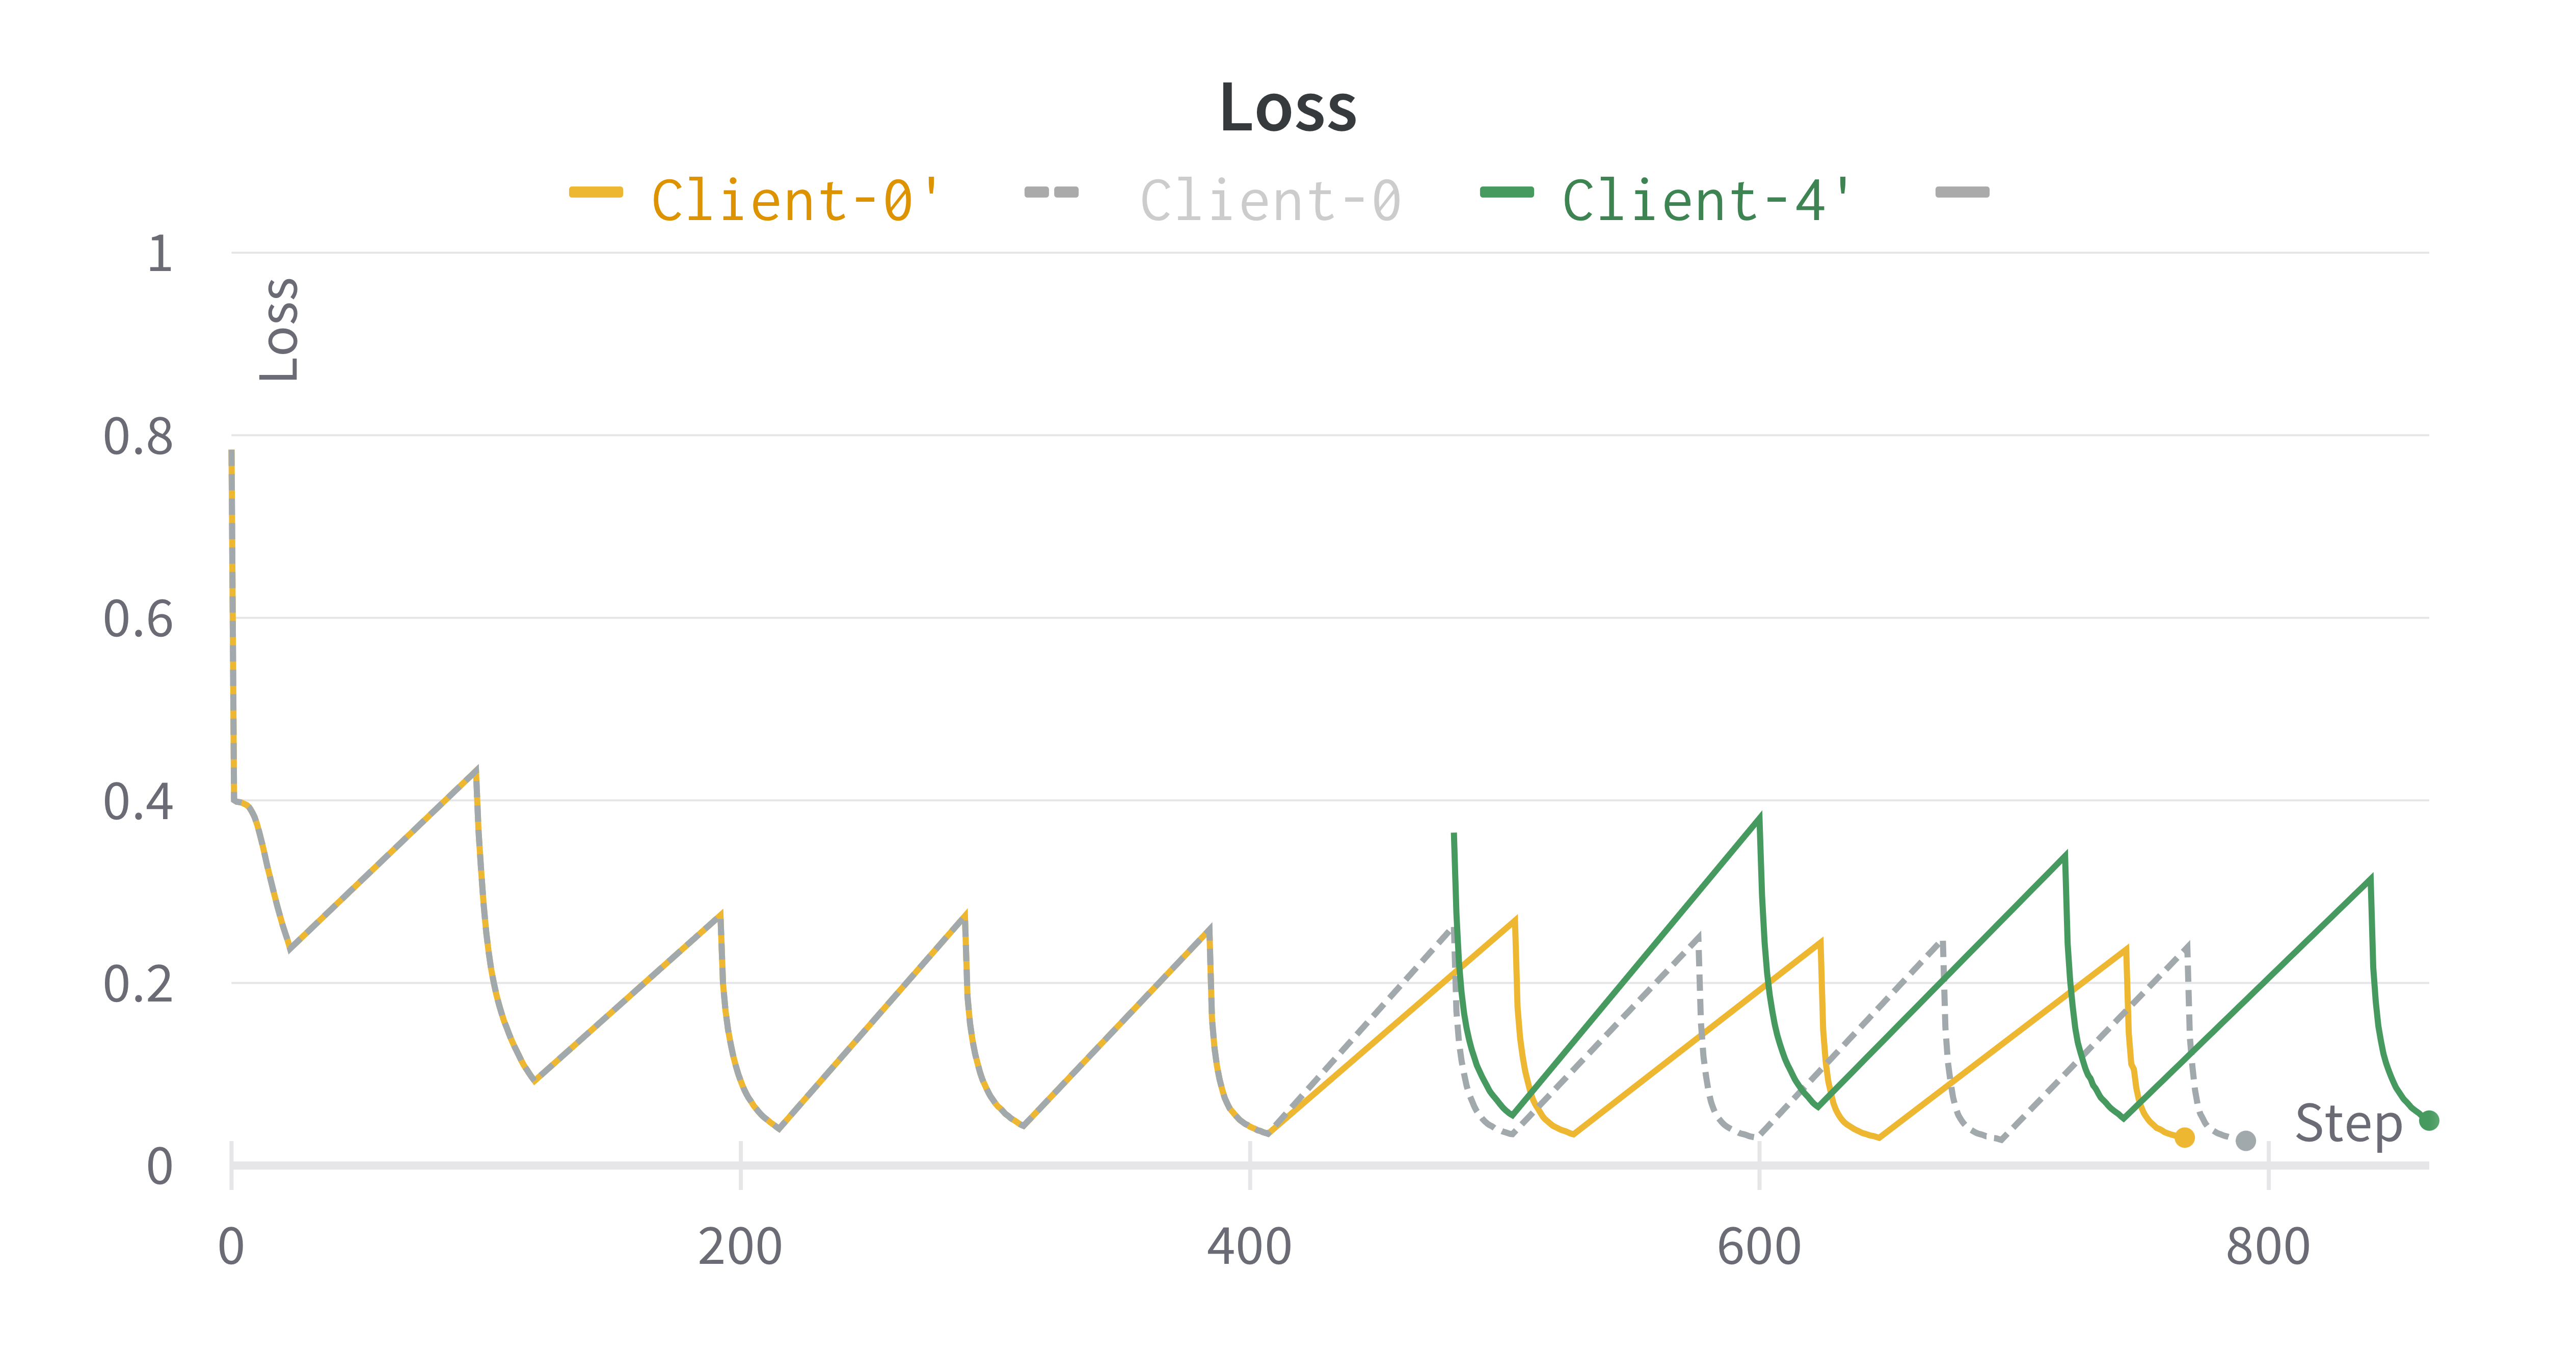
\includegraphics[width=0.75\textwidth]{figures/add-5-client.png}
  \caption{联邦学习中新增客户端节点}\label{fig:add-5-client}
\end{figure}

其中实线为新增客户端节点的实验乙数据,虚线为实验甲数据。从图中不难看出,对于0号客户端节点,实验甲和乙两次对比实验均收敛,即引入新客户端节点后,模型收到的影响不大。对于实验乙的新增客户端节点,其初始化模型基本已经收敛,表现了分布式的联邦学习能有效减少新增客户端节点的模型训练时间。

\section{本章小节}
本章阐述了联邦学习范式,并研究了联邦学习全局聚合优化算法和通讯压缩方法。为了在有限条件下,验证联邦学习用在缺陷检测算法上的可行性,本章引入了联邦学习仿真框架,并在其上进行了分布式缺陷检测部署实验。实验结果表明,应用联邦学习可以实现实时性和拓展性好的分布式缺陷检测。